\section*{Background}

\begin{frame}{CSV file format}
    \begin{minipage}{0.40\textwidth}
        \begin{itemize}
            \item[-] Easy for storing data in \dquote{tabular} format;
            \item[-] Human readable;
            \item[-] can be read by tabular softwares (\ie{} Excel, LibreOffice Calc);  
        \end{itemize}
    \end{minipage}\hfill%
    \begin{minipage}{0.59\textwidth}
        \begin{figure}
            \centering
            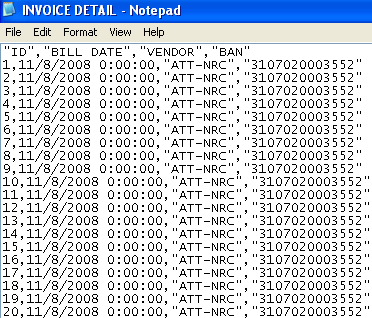
\includegraphics[width=1.0\textwidth]{{src/images/csv}}
        \end{figure}
    \end{minipage}%
\end{frame}

\begin{frame}{Background and technologies used}

    \begin{minipage}{0.48\textwidth}
        \begin{itemize}
            \item Language: Python 3[.6]: duck typing, scripting, \code{ABC} library, usually installed by default;
            \item ArangoDB: NoSQL graph-based database; basically we can store \code{JSON}; Compactly represent data;
            \item Pandas: allows operations on \dquote{dataframe} ($\approx$ CSV);
        \end{itemize}
    \end{minipage}\hfill%
    \begin{minipage}{0.48\textwidth}
        \begin{figure}
            \centering
            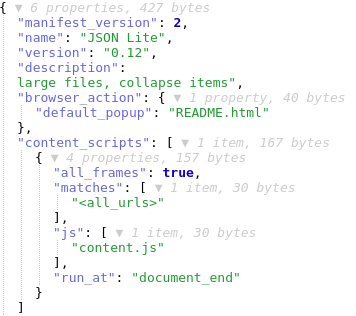
\includegraphics[width=1.0\textwidth]{{src/images/json}}
        \end{figure}
    \end{minipage}%

\end{frame}

\begin{frame}{Design Patterns}
    \begin{itemize}
        \item template: abstract class provides general behaviour with an concrete unmodifiable method $m$ whilst derived classes implements single tasks used in $m$ (\eg{} \code{java.awt.Component});
        \item Interface: allows usage of methods from a not-well specified object abstracting from its actual implementation;
        \item API: a method or a service a library or a third-party system provides to the developer in order to perform a task;
    \end{itemize}
\end{frame}